\section{Algorytm rekonstrukcji ścieżki powrotnej}
\label{sec:rtrwca}
Problem śledzenia aktualnego położenia na przykładzie robota mobilnego jest często poruszany. W poszukiwaniu rozwiązań tego problemu badacze oraz inżynierowie rozwinęli szeroką gamę systemów, sensorów i technik wyszukiwania aktualnej pozycji robota mobilnego. Można wyszczególnić siedem kategorii systemów do pozycjonowania:
\begin{enumerate}
  \item Pozycjonowanie relatywne:
  \begin{itemize}
    \item odometria
    \item nawigacja inercjalna
  \end{itemize}
  \item Pozycjonowanie absolutne:
  \begin{itemize}
    \item wykorzystanie kompasów magnetycznych
    \item pozycjonowanie z zewnętrznym sygnałem nawigacyjnym (Active Beacon)
    \item system globalnego pozycjonowania (GPS)
    \item nawigacja przy pomocy zewnętrznego znacznika (Landmark Navigation)
    \item wykrywanie pozycji na podstawie przygotowanych map (Map Matching)
  \end{itemize}
\end{enumerate}
Poniżej zostaną pokrótce opisane wyszczególnione techniki pozycjonowania robotów mobilnych.

Odometria bazuje na obliczaniu położenia robota przy pomocy wzorów transformujących informacje o obrotach jego kół na przemieszczenie relatywne w stosunku do podłoża. Rozwiązanie wydaje się być proste w realizacji oraz skuteczne, jednak posiada kilka wad. Podczas stosowania tej metody nie jest możliwe określenie położenia robota gdy nie dotyka on podłoża. Problemem jest również ślizganie się kół robota, co będzie skutkowało błędami podczas obliczania jego położenia.

Nawigacja inercjalna wykorzystuje czujniki przyspieszenia oraz żyroskopy w celu pomiaru odpowiednio przyspieszenia i prędkości kątowej robota. Dane te są następnie całkowane raz (lub w przypadku akcelerometru dwa razy) w celu wyznaczenia pozycji robota. Zaletami tej metody jest brak jakiejkolwiek zależności od świata zewnętrznego. Wszystkie pomiary są wykonywane bez użycia jakichkolwiek zewnętrznych punktów odniesienia, poza podaniem początkowej prędkości i punktu startowego robota. Niestety błędy wynikające niedoskonałości czujników oraz z całkowania, kumulują się w raz z upływem czasu. Uniemożliwia to wykorzystanie nawigacji inercjalnej w zastosowaniach, wymagających określania pozycji robota w dłuższych okresach czasu.

Kompasy magnetyczne są wykorzystywane podczas stosowania metody pozycjonowania absolutnego tj. takiego, które w przeciwieństwie do pozycjonowania relatywnego nie wymaga informacji o położeniu początkowym robota. Magnetometry stosowane w kompasach pozwalają uzyskać informacje o zwrocie i kierunku robota. Próba wykorzystania magnetometru do pozycjonowania robota w pomieszczeniach nie jest jednak dobrym pomysłem. Magnetometr jest podatny na zakłócenia pola magnetycznego, generowane przez instalacje elektryczną oraz metalową konstrukcję budynku.

Pozycjonowanie z zewnętrznym sygnałem nawigacyjnym (Active Beacon) jest powszechnym sposobem wspomagania nawigacji na statkach oraz w samolotach. Technika ta jest również wykorzystywana w komercyjnych rozwiązaniach robotów mobilnych. Polega ona na ustalaniu pozycji robota, przy wykorzystaniu sygnałów zewnętrznych, jednoznacznie określających jego położenie na podstawie odległości od nadajników. Takie podejście jest bardzo dokładne, jednak wymaga przygotowania odpowiedniej infrastruktury, która może być bardzo kosztowna.

System globalnego pozycjonowania (GPS) jest odpowiednikiem metody Active Beacon na skalę globalną. W tym przypadku infrastruktura w postaci satelitów okołoziemskich jest udostępniana między innymi przez rząd Stanów Zjednoczonych.si Eliminuje to konieczność tworzenia własnej infrastruktury tak jak w przypadku techniki Active Beacon. Niestety odbiorniki GPS nie są w stanie odebrać sygnału z satelitów wewnątrz pomieszczeń, co eliminuje tą metodę w przypadku zastosowań dla robotów mobilnych pracujących w budynkach.

Nawigacja przy pomocy zewnętrznego znacznika (Landmark Navigation) polega na wykrywaniu i rozpoznawaniu przez robota obiektów, będących kształtami geometrycznymi (np. linie, okręgi, prostokąty), których położenie jest dobrze znane lub zakodowane w samym znaczniku, np. przy pomocy kodu kreskowego lub QR Code'u\footnote{QR Code -- dwuwymiarowy kod kreskowy wynaleziony przez japońską firmę Denso-Wave w 1994 roku}. Znaczniki można podzielić na dwa rodzaje: naturalne oraz stworzone specjalnie do spełnienia wymagań postawionych przez tą metodę pozycjonowania.

Wykrywanie pozycji na podstawie przygotowanych map (Map Matching), wykorzystuje czujniki wbudowane w robocie mobilnym w celu stworzenia mapy lokalnego otoczenia. Mapa ta jest następnie porównywana z wcześniej zapisaną przez robota mapą globalną. Jeżeli robot przyporządkuje zbudowaną przez siebie mapę lokalną do elementu mapy globalnej, może na tej podstawie obliczyć swoje aktualne położenie. Zaletą tej metody, jest wykorzystywanie naturalnych struktur znajdujących się wewnątrz budynku w celu określenia położenia oraz to, że robot mobilny może sam tworzyć nowe mapy i na ich podstawie określać swoją pozycję. W celu znalezienia punktów charakterystycznych podczas porównywania dwóch map, wymagana jest duża różnorodność struktury środowiska w którym porusza się robot mobilny, co jest dużym minusem. Konieczne jest także stosowanie bardzo dokładnych czujników budujących mapy.

\subsection{Wybrane rozwiązanie}
Ostateczne rozwiązanie zastosowane w robocie Dark Explorer jest połączeniem odometrii oraz nawigacji inercjalnej. Robot wykorzystuje wbudowany żyroskop w celu określenia kierunku w którym się porusza oraz akcelerometru do określenia dystansu o jaki się przesunął. Rozwiązanie to pozwala na określenie przybliżenia pozycji relatywnej względem punktu startowego. Metoda ta została wybrana ze względu na brak konieczności przygotowywania zewnętrznej infrastruktury, co zagwarantowało uniwersalność rozwiązania.

Robot Dark Explorer został wyposażony w czujniki, które mają na celu dostarczenie
informacji niezbędnych do ustalenia toru ruchu robota. Niniejszy podrozdział
opisuje algorytm wykorzystujący dane z czujników w celu wyznaczenia trasy od
obecnego położenia do miejsca z którego robot został przyniesiony przez
operatora.

Algorytm rekonstrukcji ścieżki powrotnej składa się z dwóch części. Pierwsza z
nich odpowiedzialna jest za zapamiętywanie toru ruchu robota, druga natomiast za
odtworzenie ścieżki na podstawie zgromadzonych danych. Cały algorytm opiera się
na informacjach uzyskanych z dwóch czujników: żyroskopu oraz akcelerometru.
Czujnik przyspieszenia został zastosowany w celu określenia odległości jaką
przebył robot niesiony przez operatora. Natomiast żyroskop pozwala na uzyskanie
informacji o zmianie kierunku.

\subsection{Rejestracja trasy}
Aby możliwe stało się zrealizowanie implementacji algorytmu rekonstrukcji
ścieżki powrotnej konieczne jest w pierwszej kolejności zapamiętanie wszystkich
punktów charakterystycznych trasy po której poruszał się operator.

Pierwotnym podejściem do rozwiązania problemu wykrycia toru ruchu ciała
przenoszonego przez operatora było wyznaczanie przemieszczenia na
podstawie informacji o zmianach przyspieszenia uzyskanej z akcelerometru.
W celu obliczenia drogi po jakiej poruszało się ciało, mając jedynie informacje 
o przyspieszeniu, konieczne jest wykonanie dwukrotnego całkowania wartości 
otrzymanych z czujnika. Niestety operacja ta wymaga przeprowadzania pomiarów w
bardzo krótkich odstępach czasu w celu zminimalizowania błędów całkowania.
Nie mniej istotna jest także czułość i dokładność samego czujnika
przyspieszenia. Po wykonaniu wstępnych testów tego rozwiązania stwierdzono iż
otrzymywane rezultaty nie są zadowalające  i nie pozwalają na stworzenie
stabilnego rozwiązania w oparciu o opisywane podejście. 

Rozwiązaniem pozwalającym na uzyskanie satysfakcjonujących rezultatów okazała
się metoda wykrywania ilości kroków które wykonał operator robota podczas 
przemieszczania go w inne miejsce. Użytkownik korzystając z aplikacji
sterującej rozpoczyna proces nagrywania. Podczas wykonywania kroków, operator 
robota wykonuje mimowolne ruchy ręką w górę i w dół które są rejestrowane przez
czujniki robota. Dzięki wykrywaniu odpowiedniej sekwencji przyspieszeń jesteśmy
w stanie określić czy operator wykonał krok. Po wykryciu każdego kolejnego kroku
zapisywana jest wartość kąta pomiędzy kierunkiem ruchu z poprzedniego i obecnego
kroku. Prezentowane podejście pozwala na zapisanie całej trasy w postaci
sekwencji zmian kierunku następujących po przemieszczeniu się robota o odległość
jednego kroku. Rozwiązanie to pozwala zarejestrowanie wszystkich punktów
charakterystycznych trasy przy jednoczesnym ograniczeniu ilości danych
potrzebnych do stworzenia jej logicznej reprezentacji.

Algorytm wykrywania kroków zrealizowany został w oparciu o zainstalowany w
robocie akcelerometr trójosiowy. Szczegółowy opis zasady działania
akcelerometru oraz sposobu implementacji procedury zliczania kroków zamieszczony
został w rozdziale \ref{sec:accelometer}. Informacje na temat kąta obrotu jaki
wykonał użytkownik pomiędzy dwoma punktami charakterystycznymi trasy mogą być pobierane z jednego z dwóch
czujników. Domyślnym czujnikiem jest żyroskop, który pozwala z niezwykłą
dokładnością wykonywać pomiary prędkości kątowej, a co za tym idzie umożliwia
precyzyjne wyznaczenie kąta o jaki dokonany został obrót. Więcej informacji na
temat zasady działania żyroskopu można znaleźć w rozdziale \ref{sec:gyro}.
Sensorem zapasowym jest magnetometr. Pozwala on wyznaczyć obecną orientację 
urządzenia względem bieguna magnetycznego ziemi. Robot jest w stanie na 
podstawie danych otrzymywanych z kompasu jednoznacznie wyznaczyć kąt o jaki 
został obrócony. Z zasadami działania magnetometru oraz
napotkanymi problemami które dyskryminują ten czujnik jako podstawowy przy
rejestrowaniu i odtwarzaniu toru ruchu można zapoznać się w rozdziale
\ref{sec:mag}.

\subsection{Rekonstrukcja trasy}
Użytkownik sygnalizuje zakończenie nagrywania trasy za pomocą odpowiedniego
komunikatu wysłanego za pośrednictwem aplikacji sterującej. Robot
poinformuje użytkownika o zakończeniu nagrywania ścieżki wyświetlając na ekranie
LCD informacje na temat liczby kroków zapamiętanych w trakcie ostatniej sesji.
Następnie operator, ustawia robota na podłożu w kierunku którym robot
będzie miał wracać. Rozpoczęcie procedury odtwarzania zapamiętanego toru ruchu
rozpocznie się po wysłaniu polecenia inicjalizującego algorytm rekonstrukcji
ścieżki powrotnej. Robot korzystając z informacji dostarczanych na bieżąco z
żyroskopu oraz danych zapisanych w postaci nagranej ścieżki będzie starał się
powrócić do miejsca z którego wystartował użytkownik. Dodatkowo, jeżeli na
zapamiętanej ścieżce pojawi się przeszkoda uniemożliwiająca odtworzenie ścieżki,
zostanie ona wykryta za pomocą dołączonych czujników odległości i rozpocznie się
procedura mająca na celu uniknięcie kolizji z przeszkodą. W chwili gdy robot
ominie przeszkodę będzie starał się, jeżeli to możliwe, powrócić na oryginalną
ścieżkę ruchu. Procedura ta ma na celu zagwarantowanie, że robot prawidłowo
dotrze do miejsca z którego wyruszył. W przypadku gdy robot stwierdzi, że powrót
na oryginalną ścieżkę nie jest możliwy lub ominięcie przeszkody nie jest możliwe
procedura rekonstrukcji zostanie automatycznie zakończona. Na rysunku
\ref{fig:rtrwca_avoid_obstacle} zobrazowany został sposób ominięcia przeszkody która znalazła się
na drodze rekonstrukcji ścieżki. 

\begin{figure}[ht!]
 \centering 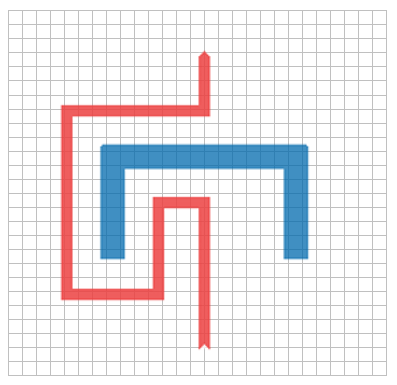
\includegraphics[height=100mm]{../images/ch04/rtrwca1.png}
 \caption{Diagram obrazujący ominięcie napotkanej przeszkody}
 \label{fig:rtrwca_avoid_obstacle}
\end{figure}

Algorytm pozwalający robotowi uniknąć zderzenia z przeszkodą opisany został ze
wszystkimi szczegółami w ramach rozdziału poświęconego czujnikom odległości. Opisany w
ramach rozdziału \ref{sec:ir-sensors} algorytm omijania przeszkód został, na
potrzeby implementacji procesu rekonstrukcji ścieżki, uzupełniony o wywoływaną w
sposób rekurencyjny metodę pozwalającą robotowi powrócić na oryginalną ścieżkę
po ominięciu przeszkody. Dodatkowym zabezpieczeniem gwarantującym zakończenie
procedury rekonstrukcji trasy, jest zatoczenie przez robota pełnego koła podczas
próby omijania przeszkód lub przekroczenie zdefiniowanego progu złożoności
przeszkody szacowanego na podstawie liczby rekurencyjnych wywołań potrzebnych do
powrotu na pierwotny tor jazdy. 
